%%%%%%%%%%%%%%%%%%%%%%%%%%%%%%%%%%%%%%%%%%%%%%%%%%%%%%%%%%%%%%%%%%%%%%%
\chapter{Описание методологии диагностики}
%%%%%%%%%%%%%%%%%%%%%%%%%%%%%%%%%%%%%%%%%%%%%%%%%%%%%%%%%%%%%%%%%%%%%%%
Методология диагностики СХД основывается на онтологической модели функционирования СХД.
В  онтологической  модели  функционирования СХД используется иерархическое представление СХД, в котором каждый из вышележащих компонентов СХД состоит из одного или более нижележащих компонентов (онтологическое отношение consistOf) (рисунок ~\ref{fig:topology}).
\begin{figure}[h]
	\centering
	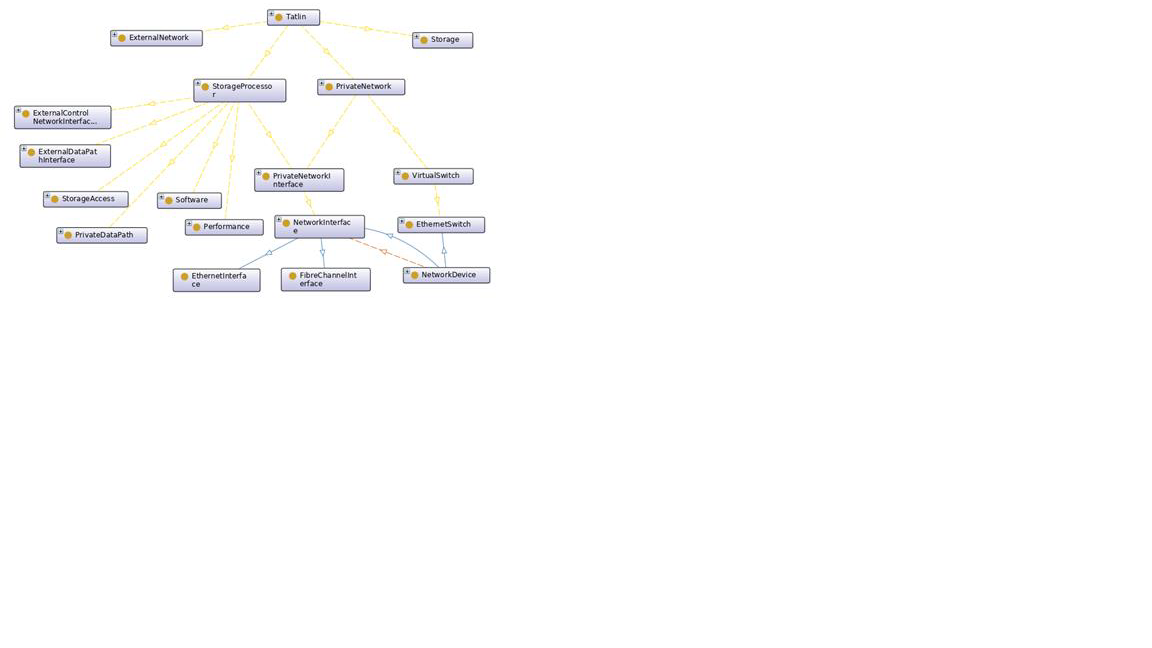
\includegraphics[width=\textwidth]{topology}
	\caption{Топология системы}
	\label{fig:topology}
\end{figure}

Каждый нижележащий компонент влияет на  состояние  вышележащего  компонента,  при  этом  степень  влияния определяется кардинальностью связи consistOf.Для поддержания работоспособности внутренней сети (PrivateNetwork) необходимо,  чтобы входящий  в  её  состав  компонент “Виртуальный коммутатор  внутренней  сети”  (VirtualSwitch)  находился  в  работоспособном состоянии,  в  то  время  как  для  нескольких  интерфейсов  подключения контроллера  к  внутренней  сети–PrivateNetworkInterface(количество интерфейсов  равно  числу  контроллеров),  достаточно  лишь  большей  части работоспособных.

На  самом  нижнем  уровне  топологии  располагаются  элементарные компоненты  (ElementaryComponent).  Каждый  элементарный  компонент связан  только  с  одним  параметром,  на  основе  которого вычисляется состояние элементарного компонента.Таким  образом,  алгоритм  диагностирования СХД включает  в  себя решение двух подзадач:
\begin{itemize*}
	\item{оценку состояния  элементарного  компонента  на  основе  значения связанного с ним параметра;}
	\item{восстановление состояний вышележащих компонентов (в том числе системы в целом) на основе состояний нижележащих компонентов.}
\end{itemize*}
Для определения состояния компонента СХД необходимо определить все  нижележащие  компоненты,  входящие  в  состав  анализируемого компонента и вычислить их состояния.Состояние СХД в целом аналогично определяется как состояние всех компонентов СХД верхнего уровня.Вычисление  состояния  компонентов  выполняется  при  помощи функции вычисления работоспособности компонента. Функция вычисления работоспособности  каждого  компонента  определена  в  онтологической модели здоровья СХД и имеет следующий вид (2.1):f = c1AND c2AND maj(c3) AND ..., (2.1)гдеа)ci–состояние компонента в домене Health: OK, Warning, Error, Fatal;б)maj(c) –функция определения состояния однотипных компонентов, связанных с исходным кардинальностью, большей 1, в простейшем случае: c31ORc32;в)AND, OR–аналоги конъюнкции и дизъюнкции для четырехзначной системы счисления.Связь  компонентов  с  параметрами  определяется  при  помощи  связиdescribedB